\chapter{Implementierung} \label{implementation}

Dieses Kapitel erläutert den Implementierungsvorgang des Java Medical Imaging Toolkits. Besonderer Wert wird auf die Umsetzung der Blattknoten wie in Kapitel \ref{architecture} Abschnitt \ref{jmedikit_structure} gelegt, da diese Anwendungsteile direkt mit dem Anwender in Aktion treten.\\
Nach einer Beschreibung wie die DICOM-Objekte repräsentiert werden, wird umfangreich auf die Bilddarstellung und Manipulation eingegangen.

\section{Implementierung der DICOM-Objekte}

Die beiden Schnittstellen \textit{IDicomData} und \textit{IDicomImageData} bilden die Grundlagen aller DICOM-Objekte die vom jMediKit erzeugt werden und sind gleichzeitig die einzige Kommunikationsmöglichkeit zu den externen Bibliotheken. Der abstrakte Adapter \textit{ADicomObject} stellt die Funktionen beider Schnittstellen zur Verfügung. Die wichtigsten Methoden stellen das Auslesen der Pixel und den einzelnen Tags eines DICOM-Objekts dar. \\
Das eingebundene \textit{dcm4che} bietet neben der Verarbeitung von DICOM-Objekten auch eine Implementierung des Kommunikations- und Speicherstandards von DICOM an. Während der aktuellen Entwicklung wurde allerdings nur ein Bruchteil der DICOM-Verarbeitung zur Erfüllung der Anforderungen benötigt und der Kommunikations- und Speicherprozess fand keine Beachtung. Bei einer Implementierung sollte dennoch eine zukünftige Erweiterung im Auge behalten werden. Dabei soll ebenso das Open-Closed-Prinzip Beachtung finden.\\
Hierbei werden die Schnittstellen in fachspezifische Domänen eingeteilt. Das bedeutet \textit{IDicomData} ist für das Verarbeiten der Tags zuständig, während \textit{IDicomImageData} ausschließlich Bilddaten verarbeitet. Für weitere Versionen können weitere Domänen implementiert werden, wie zum Beispiel eine Schnittstelle \textit{IDicomNetworkData}. Der Adapter vereint die Domänen zu einem vollen DICOM-Objekt. 

\section{Der DicomBrowser}
Der DicomBrowser ist der zentrale Part zum Transfer der DICOM-Dateien aus dem Dateisystem zu les- und verarbeitbaren DICOM-Objekten. Abbildung \ref{dicombrowser} zeigt die Darstellung nach dem Einlesenen eines Ordners mit DICOM-Dateien. Die Repräsentation entspricht dem ER-Modell aus Kapitel \ref{grundlagen} Abschnitt \ref{grundlagen:iod}. Der Knoten $\backslash$ symbolisiert die Wurzel. \textit{BRAINX}\footnote{Beispieldatensätze verfremden die tätslchlichen Patientennamen. Originale Datensätze hätten die Form \textit{Nachname\^{}Vorname}} steht für den Patientenname, gefolgt von in diesem Beispiel einer Studie, die wiederum aus sieben Serien besteht. Die einzelnen DICOM-Objekte als Blattknoten werden aufgrund der Übersichtlichkeit nicht angezeigt.\\
Die Repräsentation der Dateien ist nicht immer geordnet wie es das ER-Modell vorgibt und man kann nicht von einer sortierten Ordnerstruktur ausgehen. Die PACS-Software \textit{dcm4chee} ordnet die Daten beispielsweise nach dem Aufnahmedatum. Es wird eine Datenstruktur benötigt, die der DICOM Object Definiton entspricht.

\begin{figure}[htbp]
  \vspace{0.5cm}
  \centering
  \fbox{\includegraphics[angle=0,width=9cm]{./img/dicombrowser.png}}
   \caption{Die Baumansicht des DICOM-Browsers mit geladenen Objekten}
  \label{dicombrowser}
  \vspace{0.5cm}
\end{figure}

\subsection{Die Baumstruktur} \label{treestructure}
Sowohl die Anzeige, als auch die interne Behandlung der Daten soll so nah wie möglich an den DICOM-Standard angelehnt sein und unabhängig von der Auslieferung\footnote{Unabhängig davon, ob Dateien von der Festplatte geladen oder über das Netzwerk bezogen werden.} der Dateien die Struktur des ER-Modells haben.\\
Ein Baum als Datenstruktur erfüllt die grundlegende Repräsentation mit den verschiedenen Knotentypen aus Patientenname, Studien, Serien und den DICOM-Objekten.\\
Dadurch ergibt sich mit der Wurzel eine Höhe von
\begin{equation}
h = max(4)
\label{baumheight}
\end{equation}
und folgende konkrete Höhen der Knotentypen.
\begin{equation}
h_{Root} = 0 \qquad
h_{Patienenname} = 1 \qquad 
h_{Study} = 2 \qquad
h_{Series} = 3 \qquad
h_{Oject} = 4
\label{heights}
\end{equation}

Der minimale Baum besteht nur aus der Wurzel und hat die Höhe $h_{min} = 0$. Nach der Multiplizität des Modells aus Abschnitt \ref{grundlagen:iod} hat der Baum, sobald ein Patientenname eingefügt wird, eine minimale Höhe von $h_{min} = 3$, da Patientenname und Study jeweils mindestens ein Kindelement enthalten. Die Breite des Baums ist unbestimmt, da Knoten eine beliebige Anzahl an Kindern besitzen können. Abbildung \ref{treeexample} zeigt einen Baum, wie er in der Anwendung repräsentiert werden könnte. Der Baum enthält alle Knotentypen von \textit{Patientname} bis \textit{Object}-Ebene.\\
Zwei Klassen des Quelltextes liefern die Basis des Baums:

\begin{itemize}
\item \textbf{DicomTreeRepository}\\
	  Diese Klasse repräsentiert den Baum. Sie enthält den Wurzelknoten, und einige graphentypische Operationen. Der Baum kann nach Knoten durchsucht werden und hat eine Funktion zum Einfügen neuer Knoten. Eine Löschfunktion wurde nicht implementiert, da der Baum nicht vom Benutzer manipuliert werden soll. Das Einfügen soll nur zum initialen Einlesen aufgerufen werden.
\item \textbf{ADicomTreeItem}\\
	  \textit{ADicomTreeItem} bilden die Knoten des Baumes. Jede Instanz besitzt eine Identifikationsnummer und kennt sowohl das Elternelement, als auch die Kindknoten. 
\end{itemize}

\tikzstyle{every node}=[draw=black,thick,anchor=south, align=center]
%\tikzstyle{selected}=[draw=red,fill=red!30]
\tikzstyle{optional}=[dashed,fill=gray!50]
\begin{figure}[htbp]
\centering
\caption{Beispielhafte Darstellung eines Baumes mit $h = 4$ in der Implementierung}
\label{treeexample}
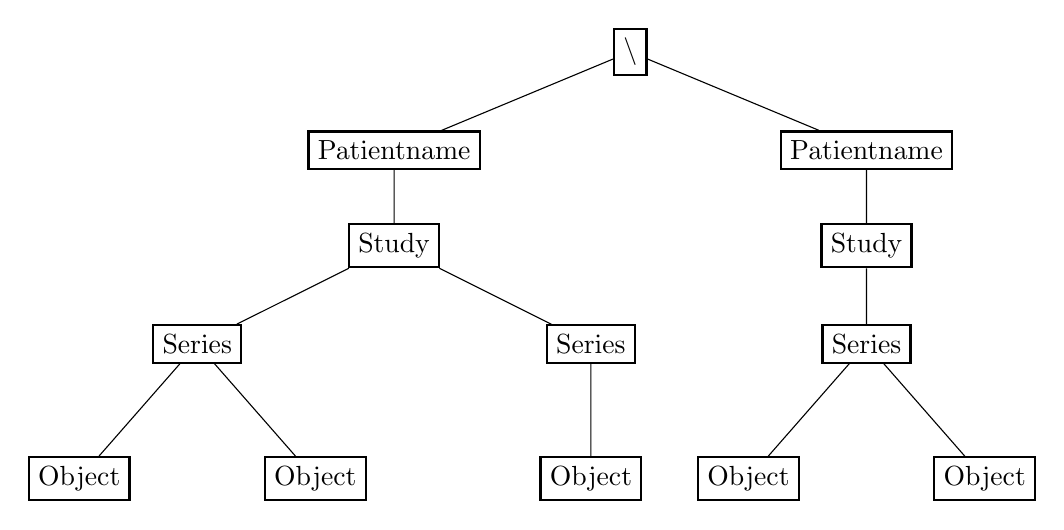
\begin{tikzpicture}[level distance=1.5cm,
  level 1/.style={sibling distance=6cm},
  level 2/.style={sibling distance=5cm},
  level 4/.style={sibling distance = 3cm, level distance = 2cm},
   level 5/.style={sibling distance=1cm},]
  \node {$\backslash$}
    child { node{Patientname}
      child { node{Study}
        child {node{Series}
        	child {node{Object}}
        	child {node{Object}}
        }
        child {node{Series}
          child {node{Object}}
        }
      }
    }
    child { node{Patientname}
    	child{ node{Study}
    	  child{ node{Series}
    	  	child {node{Object}}
    	  	child {node{Object}}
    	  }
    	}
    };
\end{tikzpicture}
\end{figure}

Da nun die Datenstruktur bestimmt ist, fehlt das Vorgehen zur Sortierung der Daten. Abbildung \ref{filesystemrep} in Abschnitt \ref{grundlagen:dicom} zeigt eine mögliche Dateistruktur. Das liefert allerdings keine Sicherheit, dass die Dateien immer vorsortiert zur Verfügung stehen. SLiegen alle DICOM-Dateien in einem Ordner, wäre eine Einteilung in Patienten und Serien etc. nicht mehr möglich.\\
Wie bereits in Abschnitt \ref{grundlagen:dicom} beschrieben besitzt jeder Patient, jede Studie und jede Serie eine eigene eindeutige Identifikationsnummer(UID), die eine modellgerechte Sortierung ermöglicht. Die Tags, die diese UIDs enthalten sind \textit{Patient ID}, \textit{Study Instace UID}, \textit{Series Instance UID} und \textit{SOP Instance UID}.\\
Jede Datei repräsentiert ein Blatt im Baum und somit ein DICOM-Objekt. Dadurch muss die abstrakte Klasse ADicomObjekt aus der Architekturbeschreibung aus Kapitel \ref{architecture} Abschnitt \ref{adapter_dependencies} angepasst werden und erweitert die abstrakte Superklasse ADicomTreeItem. Somit erben alle DICOM-Objekte die Eigenschaften eines Knoten im Baum. Zur weiteren Klassifizierung der Knoten werden die Klassen \textit{DicomPatientItem}, \textit{DicomStudyItem} und \textit{DicomSeriesItem}, die alle von \textit{ADicomTreeItem} erben, eingesetzt.
Bei der Instantiierung des DICOM-Objekts wird direkt die UID über \textit{SOP Instance UID} zugewiesen. Als nächster Schritt wird aus dem DICOM-Objekt der Pfad von der Wurzel zum Objekt ermittelt. Dazu werden \textit{Patient ID}, \textit{Study Instace UID} und \textit{Series Instance UID} des Objekts ausgelesen. Nun wird der Baum nach den entsprechenden Objekten und den UIDs durchsucht. Sind diese nicht vorhanden, wird das zugehörige Objekt erzeugt und in den Baum eingefügt, bis letztendlich das DICOM-Objekt als Blatt eingehängt werden kann.\\
Mittels dieser Sortierung entsprechen die Elemente im DicomBrowser der Darstellung des ER-Modells.


\section{Repräsentation der Pixeldaten}

Ganzzahlige Datentypen in Java (\textit{byte}, \textit{short}, \textit{int}, \textit{long}) werden im Zweierkomplement kodiert\cite[S.106]{java:insel}]. Dadurch sind nur Werte im Bereich von $[-2^{BIT-1}, 2^{BIT-1}-1]$. Das entspricht beim Datentyp \textit{short} dem Intervall von $[-2^{15}, 2^{15}-1] \rightarrow [-32768, 32767]$.\\
Medizinische Grauwertbilder besitzen meist eine Tiefe von 8-, 12- und 16-Bit. Zusätzlich bestimmt der DICOM-Tag \textit{PixelRepresentation}, ob Pixelwerte vorzeichenbehaftet sind. Durch diese variablen Eigenschaften entstehen unterschiedliche Bildtypen. Aus dem Abschnitt \ref{grey_images} wird deutlich, dass Grauwertbilder mit einer Tiefe von 16-Bit den Bereich von $[0,65535]$ abdecken. Dadurch entsteht eine Diskrepanz zwischen dem 16-Bit Java Datentyp \textit{short} und den Grauwerten. Die Pixelwerte können vom Typ \textit{short} nicht aufgenommen werden. Das gleiche Missverhältnis entsteht bei einer Tiefe von 8-Bit. Wie in Tabelle \ref{java:datentypen} zu sehen, fasst der Datentyp \textit{byte} maximal einen Wert von 127 während der größte Pixelwert 255 entspricht. Daraus folgt, dass Grauwertbilder ohne vorzeichenbehaftete Werte (Unsigned) mit dem nächsthöheren Datentyp repräsentiert werden.

\begin{table}
    \begin{tabularx}{\textwidth}{|X|X|X|X|}
    \toprule
    \hline
    \textbf{Datentyp}         & \textbf{MIN}    & \textbf{MAX}& \textbf{Unsigned} \\ \hline
    byte 		 			  & -128					& 127 		  & 0 - 255\\ \hline
    short 		 			  & -32768				& 32767 		  	  & 	0 - 65535\\ \hline
    int						  & -2147483648		& 2147483647 		  & 0 - 4294967295\\ \hline
    long 				      & \tiny{-9223372036854775808}			& \tiny{9223372036854775807} 		  & \tiny{0 - 18446744073709551615}\\ \hline

    \bottomrule
    \end{tabularx}
    \caption {Ganzzahlige Datentypen in Java}
    \label{java:datentypen}
\end{table}

\begin{table}
    \begin{tabularx}{\textwidth}{|p{5cm}|X|X|X|X|}
    \toprule
    \hline
    \textbf{Klassenname}         & \textbf{Pixeltyp Code}    & \textbf{Bittiefe Code}& \textbf{Bittiefe DICOM-Objekt} & \textbf{Vorzeichen} \\ \hline
    UnsignedByteImage 		 	& short					& 16 		  & 8 & \O \\ \hline
    ShortImage 		 			  & short				& 16 		  	  & 	16 & ja\\ \hline
    UnsignedShortImage						  & int		& 32 		  & 16 & \O \\ \hline
    IntegerImage (Farbbild)				      & int		& 32, 8-Bit je Kanal		  & 32, 8-Bit je Kanal & \O \\ \hline

    \bottomrule
    \end{tabularx}
    \caption {Von jMediKit implementierte Bildtypen}
    \label{java:bildtypen}
\end{table}

Tabelle \ref{java:bildtypen} zeigt eine Darstellung der implementierten Bildtypen und die zugehörigen Datentypen der Pixel im Quelltext. Haben die Pixeldaten eines DICOM-Objekts eine Tiefe von 8-Bit und sind nicht vorzeichenbehaftet, wird zur Repräsentation in der Implementierung ein Array des Typs \textit{short} verwendet, um alle Werte aufnehmen zu können.\\
Der Datentyp \textit{int} könnte alle Pixelwerte eines DICOM-Objekts aufnehmen. So liegt es nahe, dass Integer durchgehend als Datentyp verwendet wird. Arbeitet man allerdings mit 8-Bittiefe ohne Vorzeichen, wird der Speicherbedarf von 16 auf 32 Bit pro Pixel verdoppelt. Daher ist es sinnvoll die Bildtypen zu kategorisieren.

\subsection{Räumliche Sortierung der Bilddaten}

Beim Erstellen des Baums aus Abschnitt \ref{treestructure} wird rekursiv das Verzeichnis durchlaufen und nach lesbaren DICOM-Objekten gesucht. Ist die Suche erfolgreich, wird das Objekt dem Baum hinzugefügt. Hierbei kann das Problem auftreten, dass Dateien in der falschen Reihenfolge importiert werden. So kann es passieren, dass ein Importvorgang abhängig vom Dateinamen Objekte dem Baum hinzufügt. Die räumliche Reihenfolge der einzelnen Schichten entspricht allerdings keineswegs dem Dateinamen\footnote{Je nach Sortierung innerhalb des Betriebssystems könnte ein Import auch nach dem Änderungsdatum erfolgen} oder anderen dateibezogenen Reihenfolgen. Dadurch wird, wie schon bei der Sortierung nach dem ER-Modell, eine Methode benötigt, mittels DICOM-Tags die korrekte Reihenfolge der Bilddaten herzustellen.\\
Der Standard verfügt über mehrere Tags, welche die richtige Reihenfolge andeuten. \textit{Instance Number} ist nach dem Standard \cite[C.7.6.1]{dicom:iod} eine Nummer, die ein Bild identifiziert. Während der Entwicklung entsprach dieser Wert der Testbilder der dargestellten Reihenfolge, jedoch ist keine Information enthalten ob diese der tatsächlichen Reihenfolge im Raum entspricht. So könnte der Wert für die Aufnahmenreihenfolge oder andere konsekutive auf- oder absteigende Folgen stehen. Dadurch ist \textit{Instance Number} nur bedingt geeignet.\\
Ein Tag, der räumliche Informationen enthält ist \textit{Slice Location}.Nach dem Standard \cite[C.7.6.2]{dicom:iod} ist dieser Wert die relative Position der Bildebene in mm. Es ist allerdings keine Information enthalten, ob die Sortierung in steigender oder fallender Reihenfolge erfolgt. Da der Tag zusätzlich nur optional vorhanden ist, kann eine Nutzung zur Bestimmung der Anordnung ausgeschlossen werden.
In der Mailingliste des Insight Segmentation and Registration Toolkits \cite{itk:mail} wird eine Berechnung über die Attribute \textit{Image Position} und \textit{Image Orientation} vorgeschlagen.

\begin{figure*}[htb]
%\subfigure[Keypoints]{\includegraphics[width=0.49\textwidth]{./img/basmati_keypoints.png}}\hfill
\centering
\fbox{
\subfigure[Darstellung der beiden Spannvektoren der Bildebene]{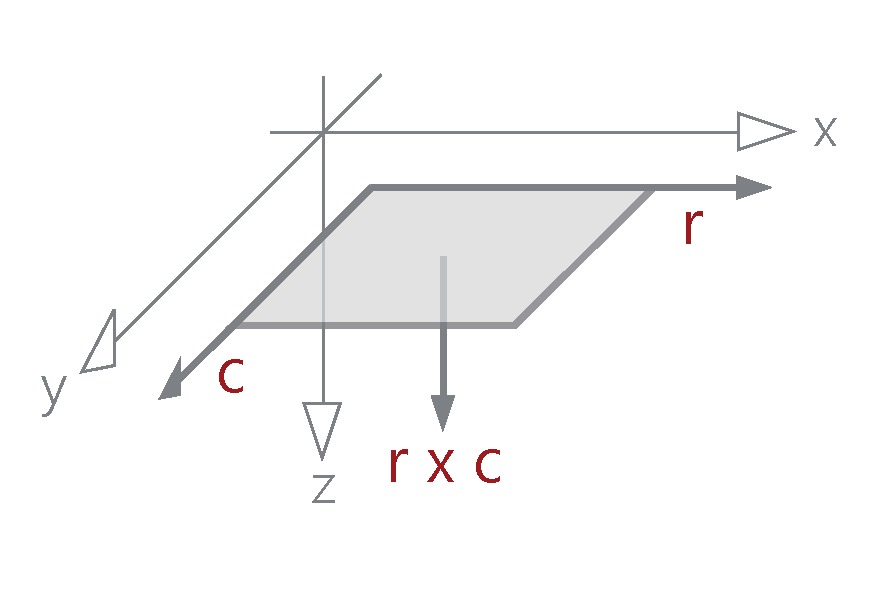
\includegraphics[width=5cm]{./img/normalenvektor.pdf} \label{sort:single}}
\subfigure[Vektoren weiterer Bildebenen]{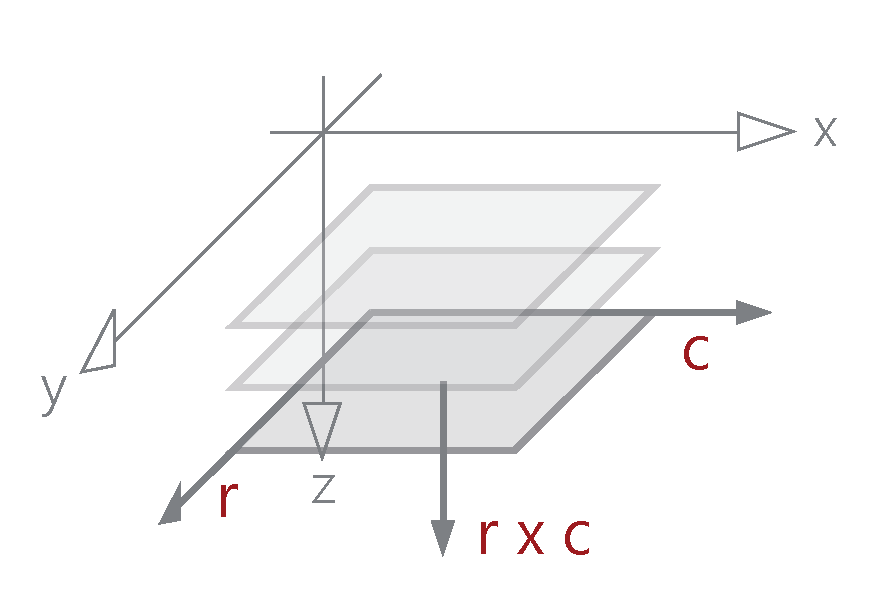
\includegraphics[width=5cm]{./img/normalenvektorstack.pdf} \label{sort:stack}}
\subfigure[Objektanordnugn an der dominanten Achse]{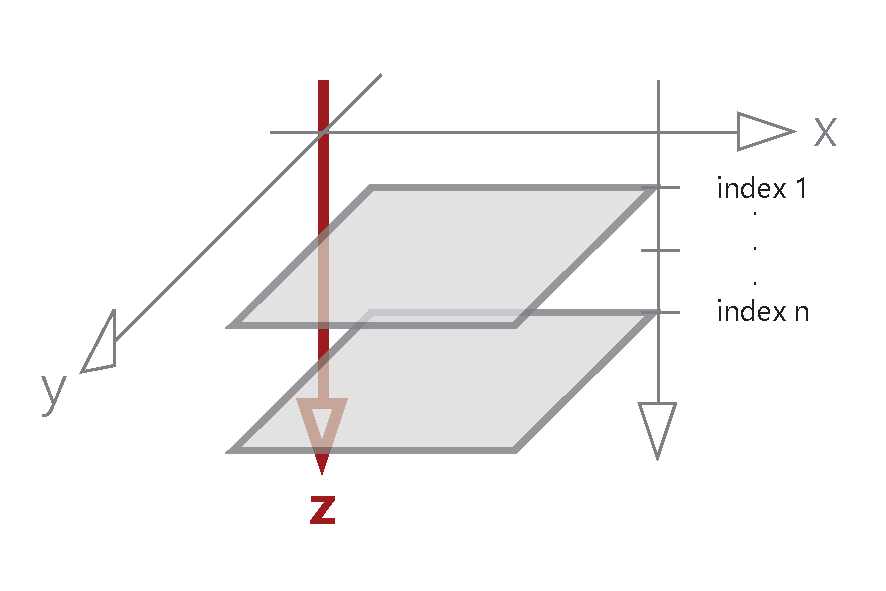
\includegraphics[width=5cm]{./img/dominantindex.pdf} \label{sort:dominant}}
}
\caption{Räumliche Sortierung der DICOM-Objekte}
\label{sort}
\end{figure*}

\section{Zeichnen der Bilddaten mit dem DicomCanvas}

Sowohl die DICOM-Objekte, als auch Bilddaten stehen im Speicher zur Verarbeitung bereit. Dieser Abschnitt befasst sich mit der Visualisierung dieser Daten.

\subsection{Implementierung der Werkzeuge}

\subsubsection{Das Bild bewegen mit dem MoveTool}

\subsubsection{Skalierung mit dem ResizeTool}

\subsubsection{Justierung der Fensterung mit dem WindowTool}

\subsubsection{Punktauswahl mit dem PointTool}

\section{Das Utility-Fenster}

\subsection{Debugging mit dem ConsoleView}

\subsection{DICOM-Objekte über DicomTagView ausgeben}

\section{Implementierung des Hauptmenüs und der Werkzeugleiste}

\subsection{Das Hauptmenü}

\subsection{Die Werkzeugleiste}



